\documentclass{article}
\usepackage{microtype}
\usepackage{graphicx}
\usepackage{subfigure}
\usepackage{booktabs}
\usepackage{hyperref}
\newcommand{\theHalgorithm}{\arabic{algorithm}}
\usepackage[accepted]{icml2018}
\icmltitlerunning{Sberbank Russian Housing Market}

\begin{document}

\twocolumn[
\icmltitle{\textit{Sberbank Russian Housing Market:} \\
    Kaggle's House Price Estimation Task with Massive Predictors}
\begin{icmlauthorlist}
\icmlauthor{Li Ziyao, 1500017776}{}
\end{icmlauthorlist}
\icmlkeywords{House Market, Kaggle, Machine Learning}
\vskip 0.3in
]

\begin{abstract}
\textit{Sberbank Russian Housing Market} \footnote{https://www.kaggle.com/c/sberbank-russian-housing-market} \footnote{The original competition was hold June, 2017. Submissions made in this report are late submissions.} is a Kaggle competition estimating deal prices in different transactions of houses. Basic house information, the neighborhood and the region information of the house, and national macro-economy data at time are provided in the dataset.

Preprocessing and feature engineering are hard work in this competition due to the low data quality. Missing values are common, and obvious inconsistencies can be found in the data. The MICE method is applied to fill some of the missing values, and delicate manual work is done for others. XGBoost\cite{xgboost}, a tool kit based on Gradient Boosting Method is applied as the main model, and Several other models are tested as well. A stack strategy for different predicted results is implemented to achieve better performance.
\end{abstract}

\section{Introduction}

Housing costs demand a significant investment from both consumers and developers. The price of a specific house not only depends on the house itself, but is also correlated with the macro house market. Sberbank, Russia’s oldest and largest bank, helps their customers by making predictions about realty prices so renters, developers, and lenders are more confident when they sign a lease or purchase a building.

Although the housing market is relatively stable in Russia, the country’s volatile economy adds to the challenge of forecasting house prices, while complex interactions between different housing features such as number of bedrooms and location are enough to make pricing predictions complicated.

The datasets provided by Sberbank contains detailed descriptions to a specific transaction: house information, a multi-perspective description of the neighborhood of a house, and a basic description of the region a house is in. Although massive predictors are introduced, none of them are dominant ones. To fully leverage these  high-dimensional predictors, ensemble methods are usually  the best choice , since features and different combinations are adequately explored in the model.

\section{Data Description}

\subsection{Data Outline}

Dataset \textit{Sberbank Russian Housing Market} is published in a Kaggle competition\footnote
{https://www.kaggle.com/c/sberbank-russian-housing-market}, of which the target is to predict accurate prices of individual house properties given information about both time and space. Each sample is a house transaction during 2013 and 2016. Hundreds of variables are given to describe the transaction, generally categorized as the following four classes:

\begin{itemize}
\item \textbf{House Description:} basic information about the house itself, including features such as  area, floor, and number of rooms, 10 features in total.
\item \textbf{Neighborhood Description:} a detailed, multi-perspective description of the neighborhood, mainly made up of numbers of specific facilities in the neighborhood, and the distance from the house to them, 207 features in total.
\item \textbf{Region Description:} a brief description of the region of the house, including features such as population, area, and whether certain kinds of facilities are in the region, 71 features in total.
\item \textbf{Macro-economy Data:} macro-economy data of the transaction time, such as CPI, GDP growth and various other economy variables, 99 features in total.
\end{itemize}

38133 samples are given in the dataset, with 30471 (80\%) labeled as training data and 7662 (20\%) unlabeled as task\footnote{Training samples are transactions before Jun. 30th, 2015, and test samples are after. That is, labeled samples are not randomly selected, and the estimation somehow can be biased.}. The performance is evaluated based on Root Mean Squared Logarithmic Error (RMSLE).

\subsection{Missing Values}

Missing values are commonly seen across the dataset, some of which are due to invalid data such as percentage variables with denominator 0 and others are data not in hand.

Figure~\ref{fig1} shows the percentage of missing values in each feature. All three types of features suffers greatly from missing data, macro-economy data the most.

\begin{figure}[ht]
\vskip 0.2in
\begin{center}
\centerline{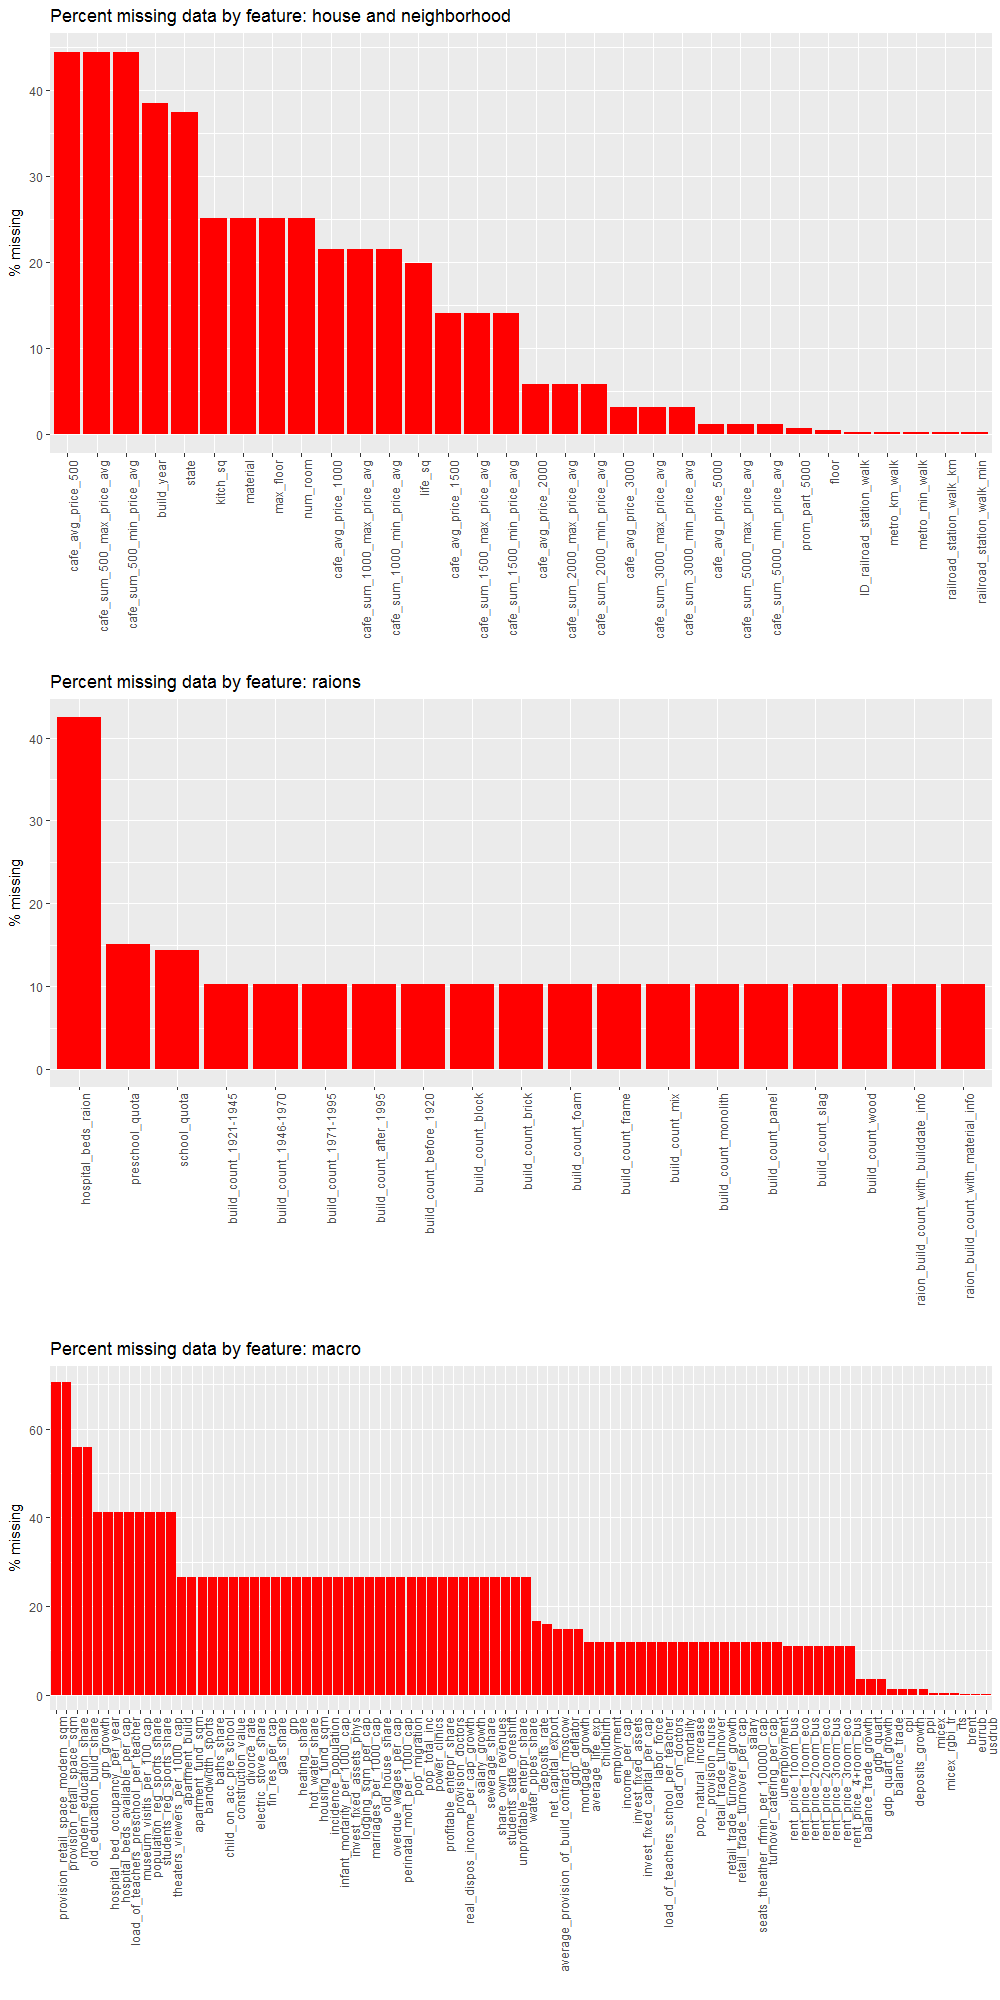
\includegraphics[width=\columnwidth]{missing}}
\caption{Missing rate of different features in house, region and macro-economy data.}
\label{fig1}
\end{center}
\vskip -0.2in
\end{figure}

\subsection{Distribution}
Figure~\ref{fig2} shows some basic distributional characteristics of the target variable \textit{price\_doc}.

According to the scatter plot, the house area is a good dominator of the house price, but only a linear upper-bound can be expected\footnote{Except for an obvious outlier.}. General idea of the good linear relationship between house price and house area is not obvious from the scatter plot, let alone a multivariate normal assumption.

According to the histogram, house price is severely right-skewed, which is common in price variables. Taking a logarithmic transformation is usually useful in regression tasks on such variables, since the logarithmic variable is usually distributed closer to a normal distribution.

\begin{figure}[ht]
\vskip 0.2in
\begin{center}
\centerline{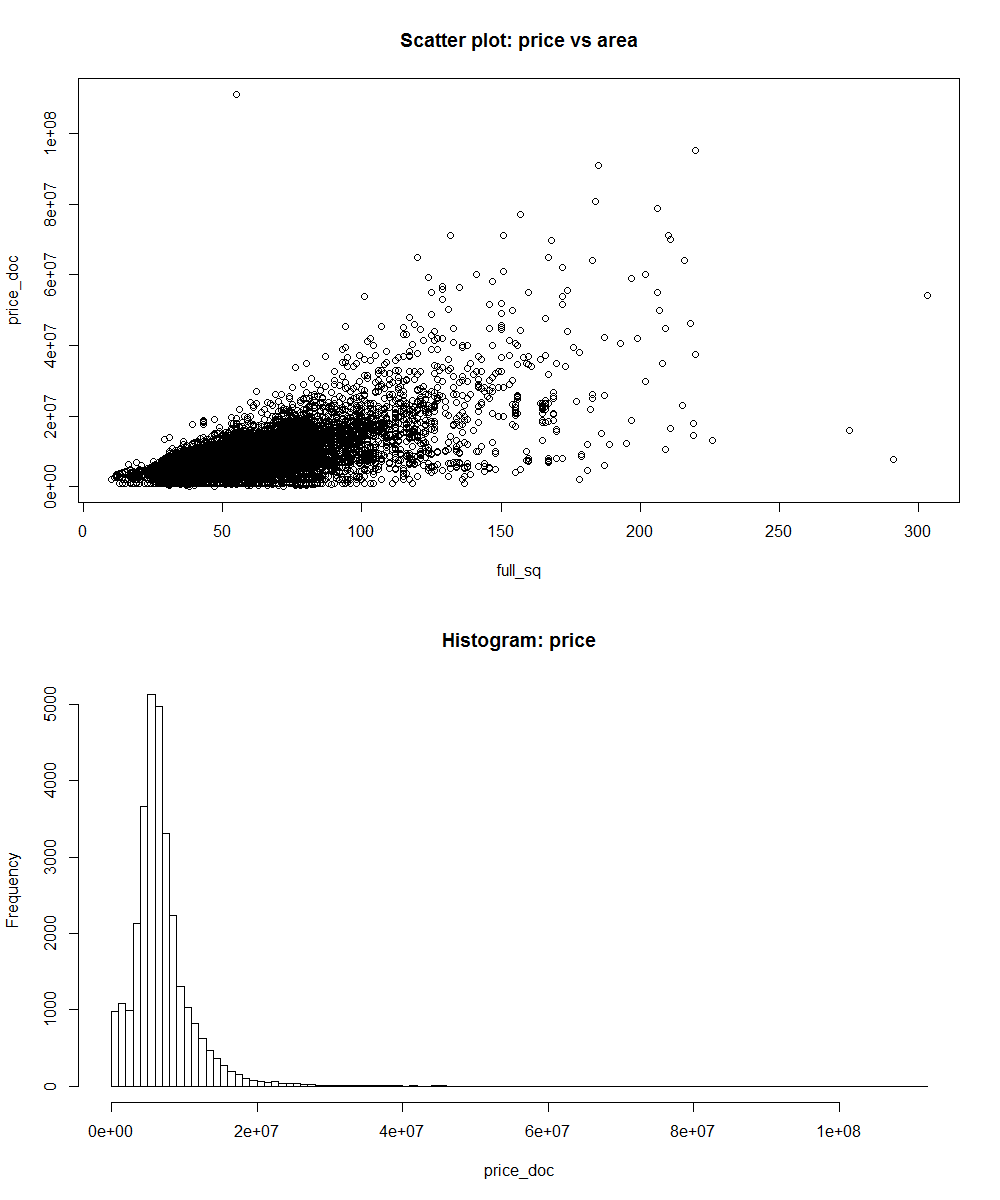
\includegraphics[width=\columnwidth]{distrib}}
\caption{A scatter plot of house price and house area and a histogram of house price. House prices distributed as a right-skewed distribution, and no clear linear relation is found between house price and house area.}
\label{fig2}
\end{center}
\vskip -0.2in
\end{figure}

\section{Preprocessing and \\ Feature Engineering}

\subsection{Preprocessing}

Preprocessing is labour-intensive in this dataset. As mentioned above, the dataset has a fair proportion of missing data, and several obvious inconsistencies and incorrect sample instances (approximately 0.1\%)\footnote{Typical inconsistencies include living area larger than full area, house floor higher than total floor of the building, etc. Typical incorrectness include 0 house area, 0 floor, etc.}.

\begin{itemize}
\item \textbf{Inconsistencies and incorrectness. } Inconsistencies are manually solved by examining the inconsistent samples one by one, looking for most promising explanations and solutions. Some of the incorrect values are manually adjusted according to corresponding values, and others are removed, leaving a missing value. Since the dataset is somehow awkwardly organized with plenty of redundancies\footnote{The original data is a merge of the four kinds of information mentioned.}, a split of different kinds of data is firstly implemented.
\item \textbf{Filling up missing values. }
    Correctly filling up the missing values is an optional\footnote{XGBoost model supports missing values, but Scikit-learn models do not.}, difficult, but sometimes instructive task. Missing values can be categorized with missing reasons into three types: some 0s are omitted in the data, some values cannot be calculated (mostly proportions divided by 0s) and some values are out of knowledge. The second type is filled with average proportion\footnote{A better way is to fill with average logit proportions, but the difference is not significant.}, and the third type is filled implementing MICE \cite{MICE} algorithm. While implementing MICE, only the features of the same categories are considered.
\item \textbf{Outliers. }
    The cause of outliers are mainly because of incorrect data, most commonly caused by omissions of decimals and typing faults. Such outliers are fixed manually. Other outliers are removed with a conservative strategy.
\end{itemize}

\subsection{Feature Engineering}

It is commonly believed that the feature engineering determines the upper-bound of a prediction, and good models approximate closer to it. Feature engineering in this task is tricky since massive heterogeneous predictors are provided. Complex structures of interactions may underlies the data.

\begin{itemize}
\item \textbf{Categorical variables. }
    Simply transforming categorical variables into one-hot encoded features is usually not recommended in high dimensional data. The categorical mean is added as an alternative. Specifically, the average house price and the average price per square-meter in a region is added as categorical features.
\item \textbf{Identical features and collinearity. }
    Several features in the dataset is almost identical. These features are removed. Features in the macro-economy data suffers severely from collinearity. Different method are attempted, namely removing 99 features to 14 independent ones \cite{kerB} and a principal components (PCA) transformation\footnote{20 principal components are selected, with $>99.99\%$ variance explained.}. Performances are similar.
\item \textbf{Changing features into proportion. }
    Several features suffers from collinearity mainly because one is a sub-feature of another. For example, the population under work age and the total population of a region. Such sub-features are replaced with proportions of the total amount. At first a drop-out-one strategy is applied, but the performance is poorer than not applying, probably shows that such collinearity is not a serious problem in ensemble methods such as XGBoost.
\item \textbf{Variables derived from timestamps. }
    House prices may fluctuate regularly during seasons, months, even weeks. Therefore, such features are extracted and added into the predictors \cite{kerB}. Experiments show that this strategy is improving the performance.
\end{itemize}

\section{Models}

XGBoost method is applied and most elaborately tuned among different models, due to its robustness and state-of-the-art performance. Other models including LASSO regression, Ridge Regression and simple neural networks are implemented as well. The results are shown in Table~\ref{tab1}.

\begin{table}[t]
\caption{Best test RMSLE of different models. }
\label{tab1}
\vskip 0.15in
\begin{center}
\begin{small}
\begin{sc}
\begin{tabular}{lr}
\toprule
Models & Test RMSLE  \\
\midrule
XGBoost & .32466 \\
LASSO & .48908 \\
Ridge & .36890  \\
Neural Network & .48644 \\
\bottomrule
\end{tabular}
\end{sc}
\end{small}
\end{center}
\vskip -0.1in
\end{table}

Simple linear models cannot achieve good performance without more manual work on feature engineering, since the high dimension of the data and reduced but still remaining collinearities. The massive hyper-parameters in network structure and poor performance on feature selection limit the performance of neural network. None the less, despite the strategies applied to prevent overfitting, such as drop-out layers and early-stopping training, the loss on the train data is still significant smaller than on the validation data. This also leads to poor performance.

XGBoost method out-performed other methods, due to its robustness and ensemble strategies, as long as its early-stopping strategy to prevent overfitting. However, training an XGBoost model, although fastest among different Gradient Boosting realizations, is still time-costing, and the hyper-parameters are so crucial to the model that a well-tuned model can out-performs a poorly-tuned one ten times or more. Massive efforts are put in parameter tuning when implementing such methods. By the way, XGBoost also out-performs the Gradient Boosting in scikit-learn package\cite{sklearn} in their best performances. The parameters of the best XGBoost model is given in Table~\ref{tab2}.

\begin{table}[t]
\caption{Best XGBoost model parameters. }
\label{tab2}
\vskip 0.15in
\begin{center}
\begin{small}
\begin{sc}
\begin{tabular}{lc}
\toprule
Parameter & Value \\
\midrule
$\eta$ & 0.01 \\
Max Depth & 8 \\
Min Child Split & 20 \\
Training Iteration & 1000 \\
Sub-sample Rate & 100\% \\
Feature Sample Rate & 50\% \\
\bottomrule
\end{tabular}
\end{sc}
\end{small}
\end{center}
\vskip -0.1in
\end{table}

Figure~\ref{fig3} shows the importance of features in the best model. According to the figure, the average price and price per square-meter variables transformed from category variables contributes significantly to the model, and Numerically encoded category features are of no significance. Good feature engineering does improve the model.

\begin{figure}[ht]
\vskip 0.2in
\begin{center}
\centerline{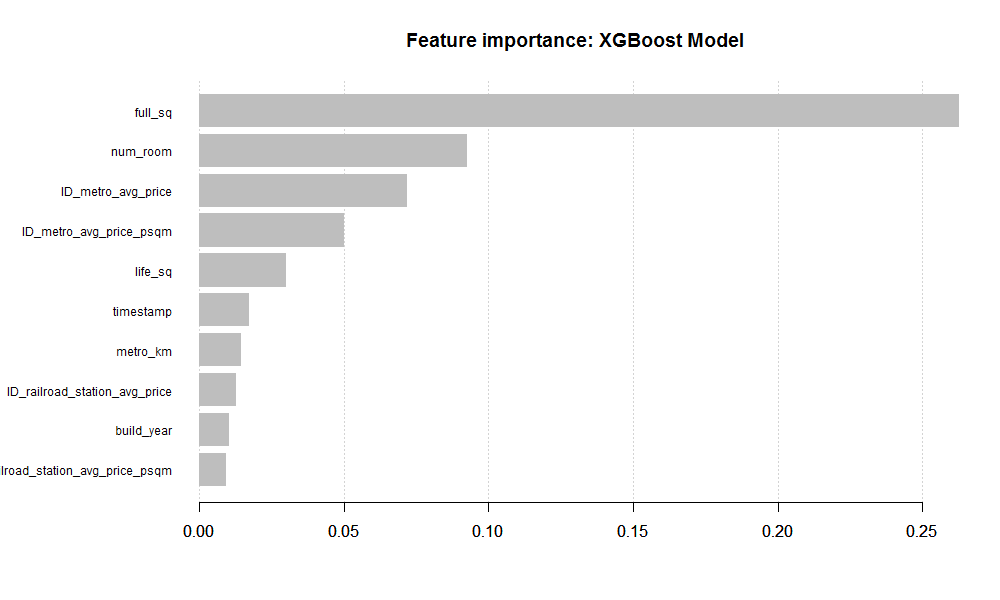
\includegraphics[width=\columnwidth]{importance}}
\caption{The top 10 important features and their corresponding importance. House area (\textit{full\_sq}) indeed is the most important effect, while metro and railroad, indicating the precise location of the property, are also important. }
\label{fig3}
\end{center}
\vskip -0.2in
\end{figure}

\section{Stacking Strategy}

Prediction from a single model may be good enough in practice, but not enough in a competition. Stacking strategies are widely implemented in Kaggle competitions. Such strategies find a best linear combination of the predicted results from different models with regard to predicting the true values.

Typical realizations of stacking strategies are regression models taking fitted values of different models as predictors and true values as target. Simple linear regression and Deep Neural Network are commonly implemented. However, in competitions with mean squared error as the evaluation method, a trick can be applied to tune the coefficients indirectly taking the true test labels as supervision.

Denote two prediction vectors as $p_1, p_2 \in R^n$, the true value $y \in R^n$, the reported Root Sum Squared Error (RSSE), derived from MSE or RMSE, as $r_1$ and $r_2$, and the Euler distance between $p_1$ and $p_2$ as $d$. Note that RSSE is equivalent to the Euler distance between a predicted value and a true value. The geometry structure of the $R^n$ space is demonstrated in Figure~\ref{fig4}. In the graph, $p \in R^n$ is a better predictor of $y$. Applying \textit{Cosine Theorem}, we have

\begin{figure}[ht]
\vskip 0.2in
\begin{center}
\centerline{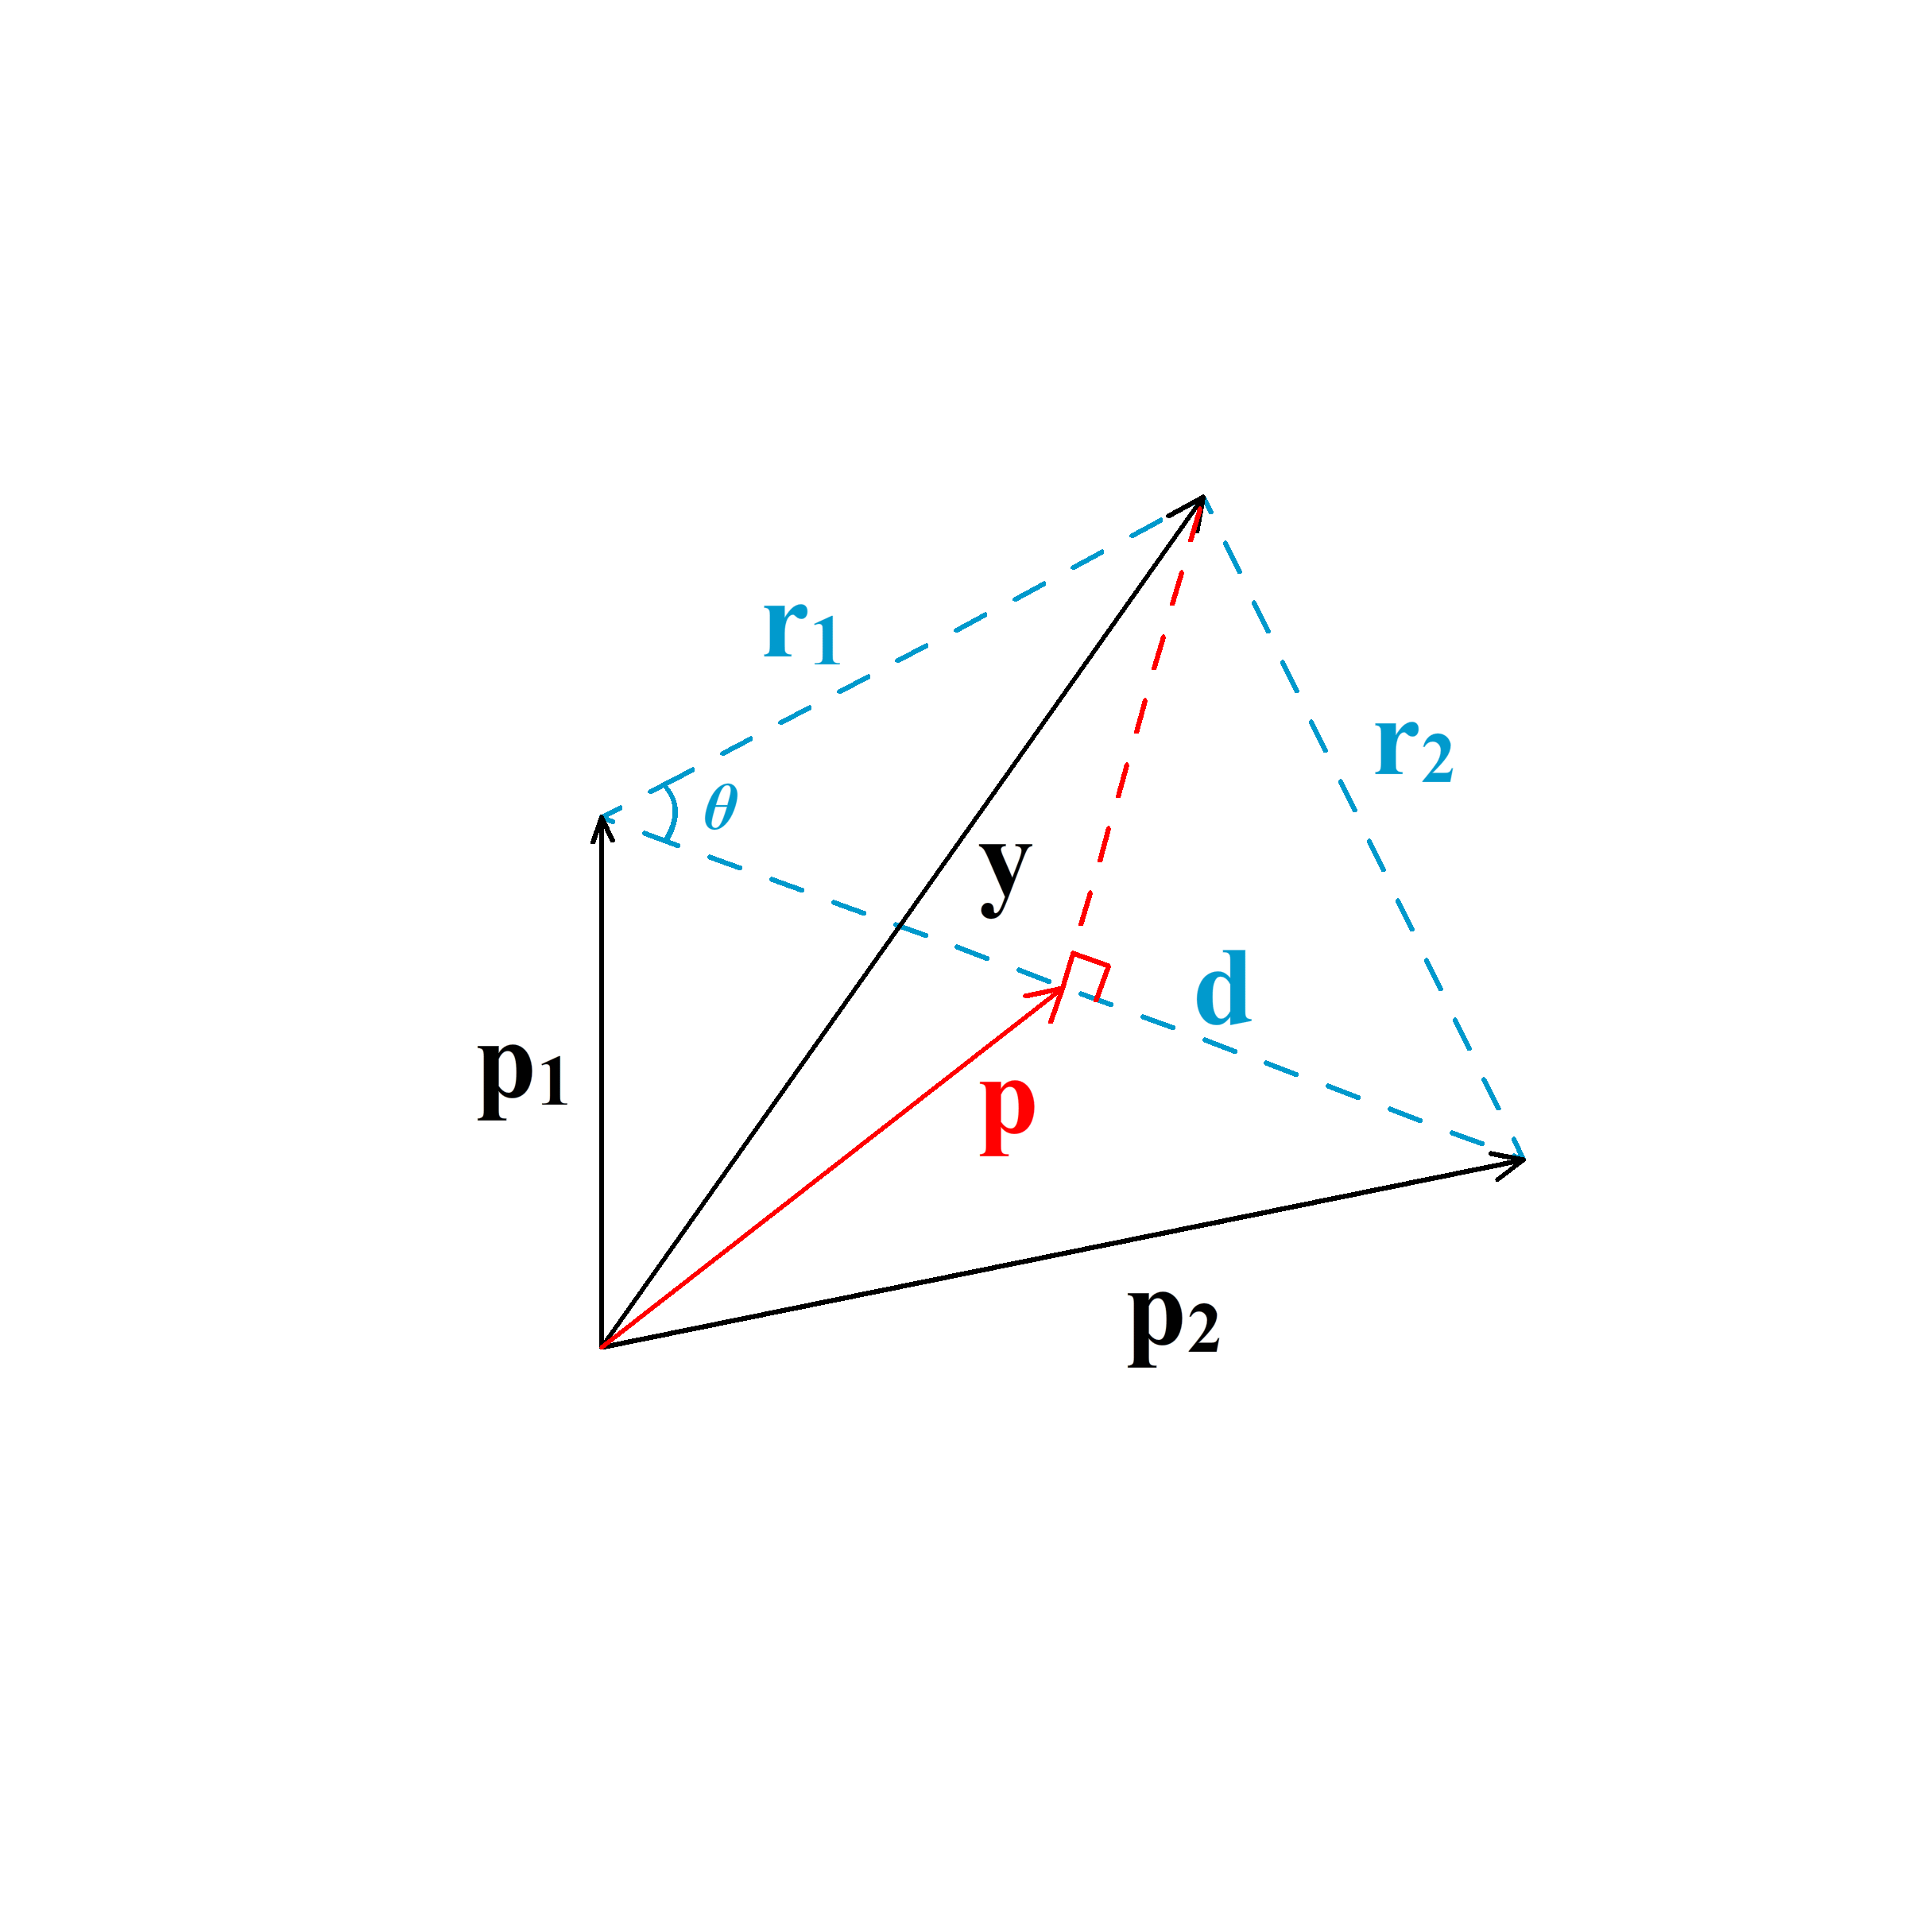
\includegraphics[width=\columnwidth]{cosine}}
\caption{The geometry structure of stacking strategy.}
\label{fig4}
\end{center}
\vskip -0.2in
\end{figure}

\begin{eqnarray*}
% \nonumber % Remove numbering (before each equation)
  p &=& (1-\alpha) p_1 + \alpha p_2 \\
  \alpha &=& \frac{r_1}{d}\cos\theta \\
  \cos\theta &=& \frac{d^2+r_1^2-r_2^2}{2dr_1}
\end{eqnarray*}

If the reported RMSE or MSE is on the full test data, $p$ is always a better predictor than $p_1$ and $p_2$. However, Kaggle evaluation system only reports errors over a certain part of the test data, this strategy not always leads to a better performance. Still, as the partial RMSE is usually a good approximation of the total RMSE as long as the test data is homogeneously divided, this method is usually available when $d$ is not so small.

Interestingly, as different predictions made by different methods are often more different from predictions made by an identical method with different parameters, the performance improved of the former case is usually greater
than the latter case, and experiments proved so. Also, weak predictors can often achieve good performance if the predictions are distinct and \textit{not that bad}.

By applying this tricks between several models, a best prediction of \textbf{$RMSE=0.30628$} is achieved, approximately 50.68\% of the variance of the logarithmic house price\footnote{Estimated on the training set. }. The best prediction made is of the \textbf{2nd} place on the competition's public leader board, among 3274 competitors (0.06\%).

\section{Conclusion}
It seems that no fancy skills or novel methods are proposed in this report, let alone making any academic achievements. Firstly, the form of the data given is direct, and no efforts in data representations is explored. Secondly, if the goal is to obtain a better position on a leaderboard of such a competition, newly proposed methods are rarely better than old ones. Traditional machine learning skills, especially those of feature engineering and preprocessing is determinant in such competitions. More efforts made in tuning parameters are also important. Therefore, such competitions become labour-intensive work, instead of research work.

These are not only somehow the deficiency of such competitions, but also the reason that the concentration of machine learning researches are more on multi-media and more complex structures. Areas of natural language processing, community mining, image and video recognition etc. have become and are becoming more and more popular, among which the representation of such complex data becomes the hottest problem. The heat of the traditional numerical machine learning problems, on the other hand, has been reducing recent years. However, as shown in the results, neural networks are no god, and the meaning of looking for better predicting algorithm never dies.

\nocite{kerA}
\nocite{kerB}
\nocite{kerC}

\bibliography{bib}
\bibliographystyle{icml2018}

\appendix
Codes, graphs, best submissions are submitted in the appendix.

\end{document}
